
\documentclass[sigconf]{acmart}
\usepackage{xspace}
\usepackage{listings}
\usepackage{multirow}
\usepackage{array}

%\newcolumntype{L}{>{\centering\arraybackslash}m{3cm}}

% defining the \BibTeX command - from Oren Patashnik's original BibTeX documentation.
\def\BibTeX{{\rm B\kern-.05em{\sc i\kern-.025em b}\kern-.08emT\kern-.1667em\lower.7ex\hbox{E}\kern-.125emX}}
    
% Rights management information. 
% This information is sent to you when you complete the rights form.
% These commands have SAMPLE values in them; it is your responsibility as an author to replace
% the commands and values with those provided to you when you complete the rights form.
%
% These commands are for a PROCEEDINGS abstract or paper.
\newcolumntype{L}[1]{>{\raggedright\arraybackslash}p{#1}}
\newcommand{\INLINECOMMENTBOX}[3]{\colorbox{#1}{#2: #3}}
\newcommand{\CCI}[1]{\INLINECOMMENTBOX{yellow}{CC}{#1}}
\newcommand{\ARI}[1]{\INLINECOMMENTBOX{blue!30}{AR}{#1}}
\newcommand{\JPI}[1]{\INLINECOMMENTBOX{green!50}{JP}{#1}}
\newcommand{\SSI}[1]{\INLINECOMMENTBOX{red!30}{SS}{#1}}

\newcommand{\COMMENTBOX}[3]{\begin{center}\colorbox{#1}{\parbox{7cm}{#2: #3}}\end{center}}
\newcommand{\CC}[1]{\COMMENTBOX{yellow}{CC}{#1}}
\newcommand{\AR}[1]{\COMMENTBOX{blue!30}{AR}{#1}}
\newcommand{\JP}[1]{\COMMENTBOX{green!50}{JP}{#1}}
\renewcommand{\SS}[1]{\COMMENTBOX{red!30}{SS}{#1}}

\newcommand{\tigress}{{\em Tigress}\xspace}
%\renewcommand{\tigress}{{\em Obfuscator}\xspace}

\newcommand{\tigressurl}{\url{http://tigress.cs.arizona.edu}\xspace}
%\renewcommand{\tigressurl}{\url{http://obfuscator.anonymized.edu}\xspace}
\newcommand{\sourceurl}{\url{https://github.com/collberg/energyIoT}\xspace}
\renewcommand{\sourceurl}{\url{https://github.com/anonymized/energyIoT}\xspace}

\copyrightyear{2018}
\acmYear{2018}
\setcopyright{acmlicensed}
\acmConference[ICCAD '19]{ICCAD '19: International Conference On Computer Aided Design}{Nov 4--7, 2019}{Westminster, CO}
\acmBooktitle{ICCAD '19: International Conference On Computer Aided Design, Nov 4--7, 2019, Westminster, CO}
\acmPrice{15.00}
\acmDOI{10.1145/1122445.1122456}
\acmISBN{978-1-4503-9999-9/18/06}


% Submission ID. 
% Use this when submitting an article to a sponsored event. You'll receive a unique submission ID from the organizers
% of the event, and this ID should be used as the parameter to this command.
%\acmSubmissionID{123-A56-BU3}

%
% The majority of ACM publications use numbered citations and references. If you are preparing content for an event
% sponsored by ACM SIGGRAPH, you must use the "author year" style of citations and references. Uncommenting
% the next command will enable that style.
%\citestyle{acmauthoryear}

%
% end of the preamble, start of the body of the document source.
\title{Energy Profiling and Analysis of Code Obfuscation for the Internet of Things}

\begin{document}
\begin{abstract}
Code obfuscation provides time-limited protection of the confidentiality of data and software by transforming code into code that is difficult to analyze, thus making reverse engineering harder. While the literature is rife with obfuscating code transformations, their application within the context of embedded systems poses considerable challenges, due to critical resource constraints, especially energy. In this paper we study the energy and performance impact of a wide range of obfuscation techniques for embedded devices. Specifically, we use Tigress, a freely available source-to-source C language obfuscator and characterize the power consumed by transformations applied to the Mibench benchmark. Our study reveals that, while energy consumption can increase as much as 2000 times over unobfuscated code for the popular virtualization transformation, careful selection of obfuscation parameters can reduce this overhead significantly. The insights gained enable software developers to select appropriate obfuscating transformations depending on their energy budget. 
\end{abstract}
\keywords{Obfuscation, tigress, energy, RPi3, virtualize,}

\maketitle

%
% The "title" command has an optional parameter, allowing the author to define a "short title" to be used in page headers.

%
% The "author" command and its associated commands are used to define the authors and their affiliations.
% Of note is the shared affiliation of the first two authors, and the "authornote" and "authornotemark" commands
% used to denote shared contribution to the research.


%
% By default, the full list of authors will be used in the page headers. Often, this list is too long, and will overlap
% other information printed in the page headers. This command allows the author to define a more concise list
% of authors' names for this purpose.
%\renewcommand{\shortauthors}{Trovato and Tobin, et al.}



%
% A "teaser" image appears between the author and affiliation information and the body 
% of the document, and typically spans the page. 
%\begin{teaserfigure}
%  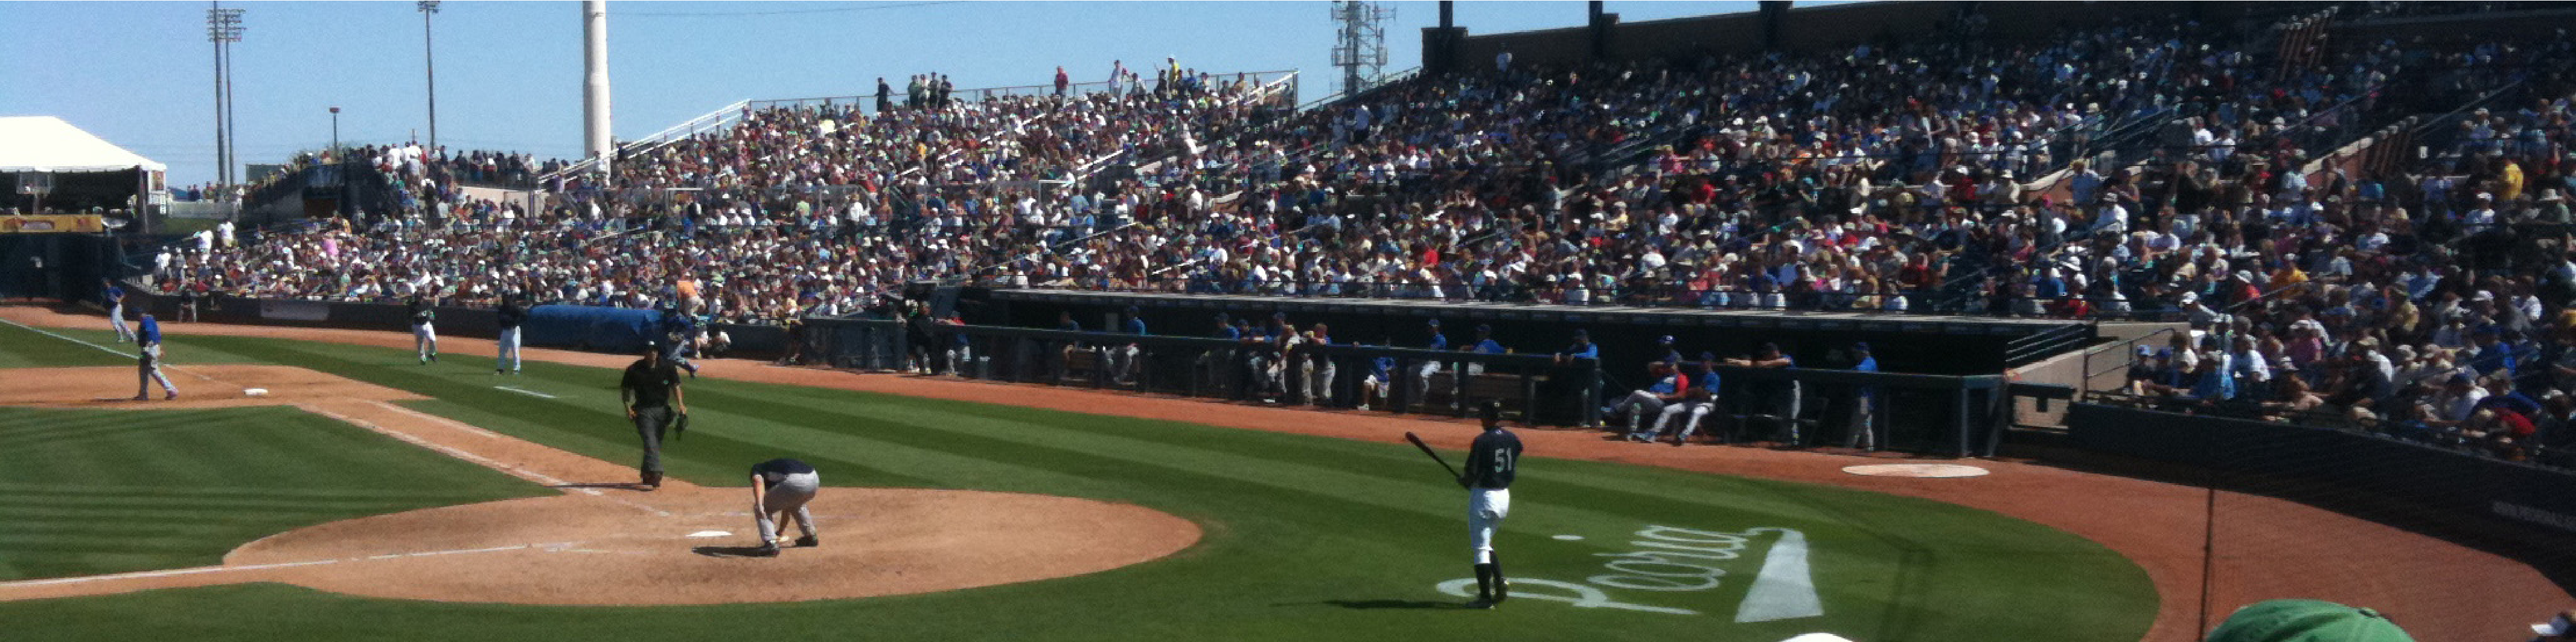
\includegraphics[width=\textwidth]{sampleteaser}
%  \caption{Seattle Mariners at Spring Training, 2010.}
%  \Description{Enjoying the baseball game from the third-base seats. Ichiro Suzuki preparing to bat.}
%  \label{fig:teaser}
%\end{teaserfigure}


\section{Introduction}
% MATE attacks against IoT devices
The Internet of Things (IoT) has seen an unprecedented growth, representing a new paradigm of devices interacting with each other, their environment, and the larger Internet~\cite{ATZORI20102787}. As these embedded devices have become ubiquitous, security and privacy have emerged as critical concerns~\cite{weber2010internet,7054433}. Since IoT devices run proprietary software and firmware and handle sensitive data, they become susceptible to attacks through tampering and reverse engineering. These types of attacks, where an adversary is in physical control of an IoT device and can manipulate its code, data, or hardware at will, are termed {\em Man-At-The-End} (MATE) attacks. 

% Software protection techniques.
Techniques to mitigate MATE attacks are termed {\em software protection} or {\em anti-tamper protection}~\cite{falcarin2011guest}. {\em Code Obfuscation} and {\em Software Tamperproofing} are popular techniques to protect code and data against MATE attacks~\cite{collberg_surreptitious_2010}. Experimental assessment of obfuscation has shown that it provides (time-limited~\cite{hohl98time}) protection against MATE attacks~\cite{5090041,7781792}.

% Performance issues for IoT devices.
It has been argued~\cite{Hosseinzadeh2015} that obfuscation can enhance code and data protection in the context of resource constrained devices as well. However, given the limited computational power available on IoT devices, any technique that purports to achieve secure computation on such devices must be evaluated with respect to its overhead: power, performance, and code size. This is a serious concern for obfuscation-based protection, as many obfuscating transformations can result in considerable computational overhead. Some prior work has addressed these issues in the context of simplistic code obfuscation techniques~\cite{6976079,dhukovic2015load,raj2017modelling}.

\subsection{Contributions}
% What we do in this work.
In this work, we study the relative impact of different obfuscating transformations on power and performance in a resource constrained environment. The ultimate goal is to make available data that will allow practitioners to select the right obfuscation technique given (a) the constraints of their hardware; (b) the characteristics of their software system; and (c) the type of asset they want to protect. Specifically, in this paper we present measurements of the energy consumption of the Raspberry Pi (RPi) running programs from the MiBench benchmark suite that have been obfuscated with the Tigress code obfuscation tool. 

Tigress~\cite{Collberg2012Distributed,banescu2015framework,banescu2016code} is a diversifying C-to-C source code obfuscator that supports a wide range of traditional obfuscating transformations. In our experimental setup we utilize the RPi as our IoT device and Tigress as our obfuscation tool. We use the MiBench embedded benchmark suite~\cite{990739} which is written in C and is designed to be representative of embedded software. We build a custom power measurement and data acquisition framework to measure the current drawn and power consumed by the various obfuscation techniques.

% Overview of rest of the paper
The rest of the paper is organized as follows. In Section~\ref{sec:related} we discuss related work in code obfuscation and IoT security. Section~\ref{sec:methodology} we describe our experimental methodology, including the obfuscating transformations we employ, and details of the experimental framework setup for power measurement and acquisition. We discuss our results in Section~\ref{sec:analysis} and outline directions for future work in Section~\ref{sec:discussion}.

% Sharing statement
{\em Sharing Statement:} The binary for the \tigress obfuscation tool can be downloaded from \tigressurl (source code is available to researchers on request). All source code, scripts, and benchmarks used to derive the results in this paper, along with raw and processed data sets are freely available to the research community at \sourceurl. 

%%%%%%%%%%%%%%%%%%%%%%%%%%%%%%%%%%%%%%%
% Old stuff
%%%%%%%%%%%%%%%%%%%%%%%%%%%%%%%%%%%%%%%
\endinput
Several works exist in literature that have analyzed and addressed the impact of security mechanisms (cryptographic algorithms and security protocols) in such devices. \CC{CITATION}   

Both open-source and commercial tools have been used to study the overall affect of obfuscation on energy, efficiency and quality of code. A taxonomy of well established obfuscation techniques was postulated~\cite{collberg1997taxonomy}. Little is studied of the impacts of these obfuscation techniques on resources relative to each other.



\section{Background and Related Work}\label{sec:related}

In this section, we review existing literature on code obfuscation, energy impact of security for IoTs in general and for code obfuscation, in particular. 

\subsection{Code Obfuscation}
\begin{figure*}
\begin{lstlisting}[mathescape=false,language=C,basicstyle=\footnotesize,escapechar=@]
int main( ) { 
  char vars[32]; union node stack[32]; union node *sp; void **pc;
  void *bytecode[1][15] =
     &&local_load_const_xor, (void *)24UL, (void *)1UL,&&local_load_const_or_const,(void *)24UL, (void *)1UL, (void *)1UL, 
     &&shiftl_minus_local_store_const, (void *)24UL, (void *)0UL, &&local_store, (void *)28UL,  &&local_load, 
     (void *)28UL, &&return_int}};
   sp=stack; pc=bytecode; goto *(*pc);
   @\underline{\tt local\_store}@: pc++; *((int *)((void *)(vars+*((int *)pc))))=(sp+0)->_int; sp--; pc++; goto *(*pc);
   @\underline{\tt local\_load\_const\_or\_const}@: pc++; (sp+1)->_int=*((int *)((void *)(vars+*((int *)pc))))|*((int *)(pc+1));
         (sp+2)->_int=*((int *)(pc+2)); sp+=2; pc+=3; goto *(*pc);
   @\underline{\tt local\_load}@: pc++; (sp+1)->_int=*((int *)((void *)(vars+*((int *)pc)))); sp++; pc++; goto *(*pc);
   @\underline{\tt return\_int}@: pc++;  return ((sp+0)->_int); goto *(*pc);
   @\underline{\tt local\_load\_const\_xor}@: pc++; (sp+1)->_int=*((int *)((void *)(vars+*((int *)pc))))^*((int *)(pc+1)); sp++; pc+=2; goto *(*pc);
   @\underline{\tt shiftl\_minus\_local\_store\_const}@: pc++; (sp+-2)->_int=((sp+-1)->_int<<(sp+0)->_int)-(sp+-2)->_int;
     *((int *)((void *)(vars+*((int *)pc))))=(sp+-2)->_int; 
     (sp+-2)->_int=*((int *)(pc+1)); sp+=-2; pc+=2; goto *(*pc);
}
\end{lstlisting}
\caption{The program {\tt int main()\{int x++;\}} obfuscated by Tigress, using first the {\tt EncodeArithmetic} transformation (which turns {\tt x++} into {\tt x = ((x|1)<<1)-(x\^{}1))} followed by the {\tt Virtualize} transformation.}
\label{fig:virtualize}
\end{figure*}

Code obfuscation has been used to mitigate several different security problems. For example, it has been used to protect security checks in Digital Rights Management systems~\cite{horning05softwarea,chow02white-box}, to protect intellectual property in languages like Java~\cite{collberg1997taxonomy}, and to diversify malware to protect it from detection by virus scanners~\cite{Skulason92mutation}. 

Collberg and Nagra~\cite{collberg_surreptitious_2010} describe many obfuscating code transformations. Common transformations include {\em control flow flattening}~\cite{wang00security} which is used to remove control flow from a function,  {\em opaque predicate insertion} which adds fake control flow statements~\cite{collberg1997taxonomy}, and {\em virtualization}~\cite{yadegari15generic}. Virtualization is a particularly common transformation, employed by many commercial tools, such as CodeVirtualizer and Themida\footnote{\url{https://www.oreans.com}.}. Figure~\ref{fig:virtualize} shows the result of virtualizing the trivial program {\tt int main()\{int x++;\}}. The virtualized code consists of a {\em bytecode} array of randomly generated virtual instructions, an execution stack, and  an interpreter specialized to execute the generated bytecode. Typically, multiple transformations are composed to protect against different types of attack. For example, the code in Figure~\ref{fig:virtualize} is the result of the {\em Mixed Boolean Arithmetic}~\cite{Zhou:2007:IHS:1784964.1784971} transformation, followed by virtualization.
\subsection{Energy impact of Security for IoT Devices}

Ensuring security and privacy on devices that are constrained by power, execution time, and code size is challenging~\cite{7823334, 6970594, 5675772}. The performance impact of security protocols and cryptographic algorithms executing on constrained devices has received much attention~\cite{potlapally2003analyzing, 5983970, 1347774, 5940923}. These works analyze the impact of energy, power and performance in the context of mobile devices where battery life is the main constraint. For example. Potlapally et al.~\cite{potlapally2003analyzing} present a framework for investigating energy requirements of the SSL protocol, and asymmetric, symmetric, and hash algorithms on battery-constrained systems. The goal of their analysis of these algorithms is to develop energy-efficient implementations. The goal of the work presented here is similar, but applied to general purpose code obfuscation, rather than cryptographic algorithms.

%%%%%%%%%%%%%%%%%%%%%%%%
\endinput
This is the foundational idea for our work in analyzing the energy impact of various obfuscation techniques for IoTs.
\AR{Fixed}


%\CC{Aakarsh needs to update this. You need to say things like "In [], Bob investigates ..., and finds that ...}

The same concerns prevail while utilizing obfuscation techniques in such constraint devices, particularly IoTs, that handle sensitive data and run proprietary code requiring the need for code/data obfuscation to harden reverse engineering.
\subsection{Energy impact of Code Obfuscation}
\CC{I rewrote this section. The last
paragraph still needs a sentence: ``the authors find...".}
\AR{Fixed}

Little work has been done analyzing the impact of individual obfuscating code transformations on energy use on constrained devices. The work most closely related to the experiments presented here are references~\cite{6976079, dhukovic2015load, raj2017modelling}. 

In~\cite{6976079}, Sahin et al. examine the energy usage of different code obfuscation tools on energy usage for mobile applications. They conclude that code obfuscation has only minor impact on battery life of mobile applications. However, their work is limited to a few  commercial obfuscation tools that mostly perform transformations unlikely to have much impact on performance, such as variable renaming, simple optimizations, and string encryption. Furthermore, they are targeting Java applications, rather than native code applications.

In~\cite{raj2017modelling}, Raj et al. 
examine the impact of code obfuscation on a very low-power micro controller, the STM32 Arm Cortex. They obfuscate four applications from the Mibench suite, using {\em lexical} transformations (identifier renaming), data transformations, and control flow transformations (flattening, deadcode insertion, extended loop condition, loop transdformation). The benchmarks are obfuscated by hand. The authors find that when the transformations are combined, the energy consumptions increases by up to 14\%.

In~\cite{dhukovic2015load}, Dukovi\'{c} and Varga present a methodology for evaluating the power overhead of code obfuscation using {\em load profiles}.
They use three commercial obfuscators that operate on the assembly code level, which perform transformations such as {\em instruction substitution}, {\em dead code insertion}, and {\em code transposition}. The authors analyze the power consumption pattern of code obfuscation using two benchmarks and conclude {\em Smart Assembly} to be the best code obfuscator to utilize if power is the criteria with {\em dead code insertion} being the main contribution to the power.   

\endinput

rather than a taxonomy of obfuscation techniques, and ii) they do not analyze the detailed impact of a suite of available code obfuscation techniques ~\cite{tigress} to suggest particular obfuscation techniques that can be utilized for resource-constrained devices. 
In this paper, we fill this gap by analyzing the energy impact of various obfuscation techniques in order to suggest the use of specific obfuscation techniques provided a given energy constraint.  




\section{Methodology}
\label{sec:methodology}
In this section, we describe our experimental set-up, including the hardware and software platforms on which our experiments were run. We also describe the obfuscating transformations that applied, and the benchmarks to which they were applied.

\subsection{Obfuscating Transformations}



% Please add the following required packages to your document preamble:
% \usepackage{multirow}
\begin{table*}[p]
\caption{Tigress transformations and transformation options used in the experiments.}
\label{tab:tigress}
\begin{tabular}{|p{2.25cm}|p{4cm}|p{11cm}|}
\hline
\multicolumn{1}{|c|}{Transformation} & \multicolumn{1}{c|}{Description}                                                                                                                                                                                                                                                                        & \multicolumn{1}{c|}{Options}                                                                                                                                                                                                                                                                                                                             \\ \hline
\multirow{3}{*}{AddOpaque}           & \multirow{3}{4cm}{Split statement sequences by adding if-statement, protected by opaque predicates~\cite{collberg98manufacturing}.} & \underline{Count} \{1,5,10,15 and 20\}: Number of opaques to add to each function                                                                                                                                                                                                                                                                                             \\ \cline{3-3} 
                                     &                                                                                                                                                                                                                                                                                                         & \underline{Kinds} \{true,bug,call,junk\}: Insertion of bogus computation allowed. Where true is the real statement, bug is a buggy statement, call is a random function and junk is random bytes.                                                                                                                                                                     \\ \cline{3-3} 
                                     &                                                                                                                                                                                                                                                                                                         & \underline{Structs} \{list, array\}: Generate opaque expressions using linked lists or arrays.                                                                                                                                                                                                                                                                       \\ \hline
EncodeArithmetic                     & Replace integer arithmetic expression with more complex expression.                                                                                                                                                                                                                  &                                                                                                                                                                                                                                                                                            \\ \hline
EncodeLiteral                        & Obfuscate string and integer literals with less obvious expressions.                                                                                                                                                                                                                    &                                                                                                                                                                                                                                                                                               \\ \hline
\multirow{6}{*}{Flatten}             & \multirow{6}{4cm}{Remove structured control flow using the control flow flattening~\cite{wang00security}.}                                                                                                                                                                                         & \underline{Dispatch} \{call, goto, switch, and indirect\}: Specifies the dispatch method of the flattened blocks of code. For call, each block is turned into its own function, goto uses indirect goto statements, and switch uses switch statements.                                                                                                       \\ \cline{3-3} 
                                     &                                                                                                                                                                                                                                                                                                         & \underline{SplitBasicBlocks} \{true,false\}: Flatten into smaller pieces by splitting up basic blocks prior to flattening.                                                                                                                                                              \\ \cline{3-3} 
                                     &                                                                                                                                                                                                                                                                                                         & \underline{RandomizeBlocks} \{true,false\}: If true, randomize  basic block sequences.                                                                                                                                                                                                                                                                 \\ \cline{3-3} 
                                     &                                                                                                                                                                                                                                                                                                         & \underline{ObfuscateNext} \{true,false\}: If true, obfuscate the computation of the dispatch variable using opaque expressions.                                                                                                                                                                                                                                        \\ \cline{3-3} 
                                     &                                                                                                                                                                                                                                                                                                         & \underline{OpaqueStructs} \{list,array\}: Type of opaque predicate to use which.                                                                                                                                                                                                                                                       \\ \cline{3-3} 
                                     &                                                                                                                                                                                                                                                                                                         & \underline{ConditionalKinds} \{branch,compute\}: How to transform conditional branches: either normal branches computed jumps.                                                                                                                                                                                                          \\ \hline
\multirow{7}{*}{Merge}               & \multirow{7}{4cm}{Merge multiple functions together into one, adding an extra formal argument to be able to call any of the constituent functions. Useful as a precursor to virtualization.
}                                                                                                                                                                                                             & Flatten \{true\}: Flatten before merging.                                                                                                                                                                                                                                                                                                                \\ \cline{3-3} 
                                     &                                                                                                                                                                                                                                                                                                         & \underline{ObfuscateSelect} \{true,false\}: If true, obfuscate the function selection argument with opaque expressions.                                                                                                                                                                                                               \\ \cline{3-3} 
                                     &                                                                                                                                                                                                                                                                                                         & \underline{OpaqueStructs} \{list,array\}: Type of opaque predicate to use.                                                                                                                                                                                                                                                       \\ \cline{3-3} 
                                     &                                                                                                                                                                                                                                                                                                         & \underline{Dispatch} \{indirect ,goto,switch\}: The dispatch method of the flattened merge.                                                                                                                       \\ \cline{3-3} 
                                     &                                                                                                                                                                                                                                                                                                         & \underline{RandomizeBlocks} \{true,false\}: If true, flattened basic block sequences are randomized.                                                                                                                                                                                                                                                                 \\ \cline{3-3} 
                                     &                                                                                                                                                                                                                                                                                                         & \underline{Split basic blocks} \{true,false\}: If true, basic blocks will be split up into individual blocks prior to merging.                                                                                                                                                                                                                                 \\ \cline{3-3} 
                                     &                                                                                                                                                                                                                                                                                                         & \underline{ConditionalKinds} \{branch,compute\}: How to transform conditional branches: either normal branches computed jumps.                                                                                                                                                                                                          \\ \hline
\multirow{2}{*}{Split}               & \multirow{2}{4cm}{Break a large function into smaller, less conspicuous, pieces which can be further obfuscated. }                                                                                                                                                                                                           & \underline{Count} \{1,10,15 and 20\}: Number of attempts to split the function.                                                                                                                                                                                                                                                                   \\ \cline{3-3} 
                                     &                                                                                                                                                                                                                                                                                                         & \underline{SplitKinds} \{block,inside,deep,top and recursive\}: \\ \hline
\multirow{5}{*}{Virtualize}          & \multirow{5}{4cm}{Turn a function into an interpreter. The bytecode language is unique to this function. 
}                                                                                                                                                                                                                                                  & \underline{Dispatch} \{switch and indirect\}: The interpreter's dispatch method. {\em Indirect} uses {\tt gcc}'s {\em labels-as-values} to implement {\em indirect threaded dispatch}.                                                                                                                                                                                                                                                                               \\ \cline{3-3} 
                                     &                                                                                                                                                                                                                                                                                                         & \underline{SuperOpsRatio} \{0,2\}: Number of super operators~\cite{proebsting96optimizing}. If {\tt >0} randomly merges  instructions together to make highly diverse virtual instruction sets.                                                                                                                                                                                                                                                                                                      \\ \cline{3-3} 
                                     &                                                                                                                                                                                                                                                                                                         & \underline{MaxMergeLength} \{0,5\}: Longest sequence of instructions to be merged into one with superoperators.                                                                                                                                                                                                                                                                        \\ \cline{3-3} 
                                     &                                                                                                                                                                                                                                                                                                         & \underline{Performance} \{PointerStack,AddressSizeShort,CacheTop\}: Tweak performance:  AddressSizeShort uses pointer arithmetic to store instruction handler addresses in a 16-bit variable, CacheTop stores the top of stack in a register.                                                                  \\ \cline{3-3} 
                                     &                                                                                                                                                                                                                                                                                                         & \underline{Operands} \{stack, registers\}: Types of virtual instruction set operands: either (implicit) stack operands or (explicit) register operands, or both. Increases virtual instruction set diversity.                                                                                                                                                                                               \\ \hline
\end{tabular}
\end{table*}

In our experiments we use the Tigress C source-to-source obfuscator. Tigress supports a wide range of transformations, and each transformation has multiple options that controls how the obfuscated code is generated. Table~\ref{tab:tigress} shows the Tigress transformations, options, and range of option values that we used in our experiments.

\begin{figure*}
\begin{center}
\begin{minipage}{12cm}
\begin{lstlisting}[basicstyle=\footnotesize]
tigress --Seed=42 --Transform=InitOpaque --Functions=main \
   --Transform=Virtualize --Functions=foo --VirtualizeDispatch=direct \
   --Transform=AddOpaque --Functions=foo --AddOpaqueCount=20 --out=output.c input.c
\end{lstlisting}
\end{minipage}
\end{center}
\caption{Example Tigress invocation.}
\label{fig:tigresscall}
\end{figure*}

Figure~\ref{fig:tigresscall} shows a  call to Tigress to transform a C program {\tt input.c} into {\tt output.c}. This particular invocation first applies the {\tt Virtualize} transformation to the function named {\tt foo} using {\em direct} dispatch, and then adds 20 opaque predicates to the virtualized {\tt foo}. This is a very typical use of an obfuscator, applying multiple transformations to the same function, in order to protect against different types of attack. Note that a {\em seed} can be given to Tigress, which randomizes all internal decisions and allows multiple, differently obfuscated, programs to be generated from the same input program. This is used to generate a diverse set of programs, making it more difficult for an adversary to create generalized attack scripts that work across many obfuscated programs. 

In our experiments, we do not combine transformations, but only apply one at a time to each of the benchmarks. For each transformation we run all possible combinations of the values of all options shown in Table~\ref{tab:tigress}. This results in 16 variants for \emph{Virtualize}, 128 variants for \emph{Merge}, 35 variants for \emph{Split}, 75 variants for \emph{AddOpaque}, 128 variants for \emph{Flatten}, 1 variant for \emph{EncodeArithmetic} and 3 variants for \emph{EncodeLiteral}. 

We apply each transformation variant to all the functions in each benchmark. In practice, this is unrealistic; in most scenarios only security-sensitive functions are obfuscated to avoid too much overhead. For the MiBench benchmarks, however, it is unclear which part of the code should be considered ``security-sensitive,'' and we therefore transform the entire program.


After transformation, the resulting program is compiled using \texttt{gcc -O2 -lm -Wall -o obfuscated.exe obfuscated\_input.c}, and the resulting program is stripped.

\CC{Jayant: What version of gcc?.}

%%%%%%%%%%%%%%%%%%%%%%%%%%%%%%%%%%%%%%
% Old stuff
%%%%%%%%%%%%%%%%%%%%%%%%%%%%%%%%%%%%%%
\endinput

\AR{Dr.Collberg: Can you add a short description of these options? Just stating it wouldn't make send to a reviewer. Else, how about having a table for this? Transformation | Options | Description}
\subsubsection{Virtualize}
Virtualize involves transforming a function into an interpretor, whose bytecode language is specialized for the particular function specified. 



\begin{itemize}
\item \textit{--VirtualizeDispatch=[direct,indirect and switch]}.
\item \textit{--VirtualizeSuperOpsRatio=[2 and 0]}.
\item \textit{--VirtualizeMaxMergeLength=[5 and 0]}.
\item \textit{--VirtualizePerformance=[AddressSizeShort, CacheTop and PointerStack]}.
\item \textit{--VirtualizeOperands=[stack and registers]}.
\end{itemize}


\subsubsection{AddOpaque}
Split up control flow by adding opaque branches.

\begin{itemize}
\item \textit{--AddOpaqueKinds=[bug and junk]}
\item \textit{--AddOpaqueCount=[1,5,10,15 and 20]}
\end{itemize}


\subsubsection{Encode Arithmetic}
Encode arithmetic replaces integer arithmetic expression with more complex expression. Tigress currently supports one option for this transformation.

\begin{itemize}
\item \textit{--EncodeArithmetic}.
\end{itemize}


\subsubsection{Encode Literal}
This technique obfuscates string and integer literals with less obvious expression. A single option of encoding integer and string is utilized.

\begin{itemize}
\item \textit{--EncodeLiterals=[Integer and String]}.
\end{itemize}

\subsubsection{Flatten}
Remove control flow from a function.

\begin{itemize}
\item \textit{--FlattenDispatch=[switch, goto and indirect]}.
\item \textit{--FlattenSplitBasicBlocks=[true and false]}.
\end{itemize}



\subsubsection{Merge}
This transformation technique merges multiple functions together into one. The following options are supported in Tigress: 

\begin{itemize}
\item \textit{--MergeFlatten=[true and false]}.
\item \textit{--MergeFlattenDispatch=[goto,indirect and switch]}.
\item Split \textit{--MergeSplitBasicBlocks=[true and false]}.
\item Randomize \textit{--MergeSplitBasicBlocks	=[true and false]}.
\end{itemize}


\subsubsection{Split}
Split transformation breaks a function into less conspicuous pieces that are their own functions. The option utilized for this transformation is an attempt at the number of times the splitting needs to be performed. 

\begin{itemize}
\item \textit{--SplitCount=[1,5,10 and 15]}.
\end{itemize}


\subsection{Benchmarks}
\CC{Jayant: describe the benchmarks here. If we didn't use all the Mibench benchmarks, explain why. If you had to modify the, explain how and why. For example, Tigress requires a merge step, this is important since it can have performance implications (a merged program may optimize better than one with multiple modules.}
\CC{Aakarsh: help out with this since you did the merging etc.}
\CC{Below is the text that Aakarsh wrote, you can use this as a starting point.}

We utilize the widely popular MiBench embedded benchmark suite ~\cite{guthaus2001mibench} as our base programs for obfuscation. Since, MiBench is written in C, it conforms with the requirements of our obfuscator, Tigress, that works only on C code. It is to be noted that since we aim at obfuscating firmware or system code, C is the most common language utilized in the realm of embedded systems. The MiBench provides a range of benchmarks divided into Automative, Network, Office, Security and Telecom applications. We choose to utilize 5 benchmark programs from each of these applications for our obfuscation experiments viz., i)\textit{basicmath} - performs basic mathematical operations for a given set of constants, ii)\textit{FFT} - performs Fast Fourier Transform and it's inverse on an array of data, iii)\textit{SHA} - produces a 160-bit message digest secure hash from a given input, iv)\textit{dijkstra} - constructs a large graph in an adjacency matrix representation and calculates the shortest path between every pair of node, and v)\textit{stringsearch} - searches for given
words in phrases using a case insensitive comparison
algorithm.

The program in the above benchmarks consists of multiple input C files and Tigress requires these input files to be merged into exactly one C file. 

\subsection{Power Measurement and Acquisition Setup}
\CC{Jayant writes this. You can start with the text below which is what Aakarsh wrote and modify it according to the setup you used. Also include a good picture.}
\begin{figure}[t]
  \centering
%  \includegraphics[width=0.9\columnwidth, height=6cm]{exp_setup.png}
  \caption{Experimental Framework}\label{expsetup}
\end{figure}
Fig.~\ref{expsetup} describes our experimental framework to measure the power and performance characteristics of various constituent obfuscation techniques along with the data acquisition system. We utilize the Raspberry Pi which is a popular platform for low-power and low-cost computational tasks with widespread applications as our resource constraint device. With it's support for input-output peripherals, network connectivity and programmability, it is exemplary for IoT applications~\cite{maksimovic2014raspberry}. In our setup, we utilize the Raspberry Pi 2 Model B (RPi) running a 900MHz quad-core ARM Cortex-A7 CPU with 1GB RAM connected to a monitor, keyboard and mouse enabled with Internet connectivity via Ethernet. 

\CC{Jayant and Aakarsh: rewrite this to fit our current system.}
We have built a custom setup to measure the power consumption from the RPi2 based on~\cite{6976079, kaup2014powerpi} that is also shown in Fig.~\ref{expsetup}. The RPi2 is powered via a micro-USB from a stable 5V power supply. A shunt resistance of 0.1$\Omega$ is connected in series between the power supply and the RPi2 in order to measure the current drawn by the device. The voltage drop across the shunt resistance is measured by connecting the ends of the resistor to the analog input pins of the Arduino Uno, that have an inbuilt analog-to-digital (A/D) converter to obtain the digital voltage values. The current drawn $I$ = $\frac{V1 - V2}{R}$ (Fig.~\ref{expsetup}), from which the power consumed by the RPi $P$ = $V2 \times I$.

The Arduino Software IDE running on a laptop is utilized to setup the data and format to be acquired from the Arduino UNO. However, actual data acquisition is performed by the Processing\footnote{https://processing.org/} software running on the laptop that communicates serially with the Arduino. The synchronization required to start and stop power measurement of the chosen obfuscation code is controlled via an Interrupt Service Routine in the Arduino, that is triggered by an interrupt signal from the GPIO pin of the RPi. Processing writes the data acquired to files stored on the laptop.

The obfuscated target outputs generated, as in ~\ref{subsec:pdoc} are executed and power samples acquired on the laptop. The start and stop of the execution is controlled by turning ON the GPIO pin of the Raspberry Pi 2 that triggers an Interrupt to the Arduino to start data acquisition and turning OFF the GPIO pin stops acquisition.   

\subsection{Performance acquisition of obfuscated codes}\label{subsec:pdoc}
\CC{Aakarsh and Jayant: Fix this.}
\JP{Fixed.
Note : The Pi 3B+ benefited from a change to the way the system-on-chip (SoC) is attached to the circuit board, allowing it to better dissipate heat. 
And all the factors such as power draw,performance varies with different versions of Pi.
https://www.raspberrypi.org/magpi/raspberry-pi-specs-benchmarks/
}
Target output for each of the obfuscated code is generated by:\\
\textit{gcc -O2 -lm -Wall -o obfuscated\_target\_filename obfuscated\_input \_filename.c}\\

We acquire the execution time(using time command) and temperature of the generated obfuscated code binary (after stripping \footnote{https://linux.die.net/man/1/strip}).

A data file is generated which includes name, start time, average execution time (5 runs), end time and average temperature of RPi3 during execution of obfuscated codes. This data file is fed to Keysight BenchVue Power Supply application which gives output of average power during the code execution. 


\subsection{{Power acquisition of obfuscated codes}}
\JP{Fixed}
We acquire the power values by directly recording current and voltage values from Keysight provided Windows application called as Keysight Benchvue Power Supply. The calculation is done by recording current and voltage values every 0.1 second for the entire 5 times execution of the obfuscated codes.
These values are then averaged and subtracted from the idle RPi3 state power consumption of 2.2805 watts. This gives the exact average power consumed by the particular obfuscated code execution.


\subsection{Energy consumption of obfuscated codes}
\CC{Aakarsh and Jayant: Fix this.}
\JP{Fixed}
The energy consumed is deduced by $P_{avg} \times t_{avg}$, where $P_{avg}$ represents the average power consumed over the execution of the obfuscated target file and $t_{avg}$ is the average execution time. To elaborate, each execution of the obfuscated target file generates several power samples (based on the sampling rate of the SMU(which is 0.1 second in our case), which are averaged to result in $P_{avg}$. 


%\subsection{Evaluation Metrics}
%\CC{Sriram writes this. I'm not sure what's %supposed to be in this section.}



\section{Power Analysis}
\label{sec:analysis}
% Please add the following required packages to your document preamble:
% \usepackage{multirow}
\begin{table*}[!hp]
\caption{Energy results.}
\label{tab:results}
\begin{footnotesize}
\begin{tabular}{|p{1.5cm}|l|l|p{5cm}|l|p{5cm}|}
\hline
Benchmark                                                                      & \begin{tabular}[c]{@{}l@{}}Obfuscation \\ Transformations\end{tabular} & \begin{tabular}[c]{@{}l@{}}Min \\ Energy (J)\end{tabular} & Min Energy Option                                                                                                                                                                          & \begin{tabular}[c]{@{}l@{}}Max \\ Energy (J)\end{tabular} & Max Energy Option                                                                                                                                                                              \\ \hline
\multirow{7}{*}{\begin{tabular}[c]{@{}l@{}}Security - \\ SHA \\ Baseline \\ Unobfuscated \\Energy = 0.0568\end{tabular}}                                                  & Add Opaque                                                             & 0.06                                                    &  Count=1,Kinds=call,Structs=list                                                                                                                                                         & 0.87                                                    &  Count=20,Kinds=true,Structs=list,array                                                                                                                                                      \\ \cline{2-6} 
                                                                               & EncodeArithmetic                                                      & 0.11                                                    &  Kinds=integer                                                                                                                                                                           & 0.11                                                    &  Kinds=integer                                                                                                                                                                               \\ \cline{2-6} 
                                                                               & EncodeLiterals                                                        & 0.06                                                    &  Kinds=string                                                                                                                                                                            & 0.07                                                    &  Kinds=integer                                                                                                                                                                               \\ \cline{2-6} 
                                                                               & Flatten                                                                & 0.07                                                    & \raggedright Dispatch=goto, SplitBasicBlocks=true, RandomizeBasicBlocks=false, ObfuscateNext=false, OpaqueStructs=list, ConditionalKinds=branch              & 9.38                                                    &        Dispatch=indirect, SplitBasicBlocks=true, RandomizeBasicBlocks=true,  ObfuscateNext=true,  OpaqueStructs=array, ConditionalKinds=branch                \\ \cline{2-6} 
                                                                               & Merge                                                                  & 0.13                                                    & 
                                                            Flatten=true, ObfuscateSelect=true, OpaqueStructs=list, Dispatch=goto,  RandomizeBasicBlocks=true, SplitBasicBlocks=false, ConditionalKinds=branch & 1.91                                                    & Flatten=true,ObfuscateSelect=true, OpaqueStructs=list,Dispatch=indirect, RandomizeBasicBlocks=false,S plitBasicBlocks=true, ConditionalKinds=branch \\ \cline{2-6} 
                                                                               & Split                                                                  & 0.04                                                    &  Count=1,Kinds=block                                                                                                                                                                     & 0.28                                                    &  Count=5,Kinds=top                                                                                                                                                                           \\ \cline{2-6} 
                                                                               & Virtualize                                                             & 13.07                                                   & Dispatch=switch, SuperOpsRatio=2, MaxMergeLength=5, Performance=PointerStack, Operands=stack                                                    & 127.09                                                  & Dispatch=switch, SuperOpsRatio=0, MaxMergeLength=0, Performance=PointerStack, Operands=registers                                                    \\ \hline
\multirow{7}{*}{\begin{tabular}[c]{@{}l@{}}Telecom - \\ FFT \\ Baseline \\ Unobfuscated \\Energy = 0.2984\end{tabular}}                                                   & Add Opaque                                                             & 0.31                                                    &  Count=5, Kinds=bug, Structs=list,array                                                                                                                                                  & 1.26                                                    &  Count=15, Kind=call, Structs=list,array                                                                                                                                                     \\ \cline{2-6} 
                                                                               & EncodeArithmetic                                                      & 0.36                                                    &  Kinds=integer                                                                                                                                                                           & 0.36                                                    &  Kinds=integer                                                                                                                                                                               \\ \cline{2-6} 
                                                                               & EncodeLiteral                                                         & 0.33                                                    &  Kinds=string                                                                                                                                                                            & 0.36                                                    &  Kinds=integer                                                                                                                                                                               \\ \cline{2-6} 
                                                                               & Flatten                                                                & 0.20                                                    &  Dispatch=switch, SplitBlocks=false, RandomizeBlocks=true, ObfuscateNext=true, OpaqueStructs=array, ConditionalKinds=compute                                                             & 1.68                                                    &  Dispatch=call, SplitBlocks=true, RandomizeBlocks=false, ObfuscateNext=true, OpaqueStructs=array, ConditionalKinds=branch                                                                    \\ \cline{2-6} 
                                                                               & Merge                                                                  & 0.33                                                    &  Flatten=true, ObfuscateSelect=true, OpaqueStructs=list, Dispatch=indirect, RandomizeBlocks=false, SplitBlocks=false, ConditionalKinds=branch                                            & 0.93                                                    &  Flatten=true, ObfuscateSelect=true, OpaqueStructs=list, Dispatch=switch, RandomizeBlocks=false, SplitBlocks=true, ConditionalKinds=compute                                                  \\ \cline{2-6} 
                                                                               & Split                                                                  & 0.33                                                    &  Count=10, SplitKinds=block                                                                                                                                                              & 0.72                                                    &  Count=5, SplitKinds=inside                                                                                                                                                                  \\ \cline{2-6} 
                                                                               & Virtualize                                                             & 0.83                                                    &  Dispatch=switch, SuperOpsRatio=2, MaxMergeLength=5, Performance=PointerStack, Operands=stack                                                                                            & 14.27                                                   &  Dispatch=switch, SuperOpsRatio=2, MaxMergeLength=5, Performance=AddressSizeShort,CacheTop, Operands=registers                                                                               \\ \hline
\multirow{7}{*}{\begin{tabular}[c]{@{}l@{}}Automotive-\\ Qsort \\ Baseline \\ Unobfuscated \\Energy = 0.16 \end{tabular}}   & Add Opaque                                                             & 0.16                                                    &  Count=15, Kinds=junk, Structs=list                                                                                                                                                      & 0.59                                                    &  Count=10, Kind=junk, Structs=list                                                                                                                                                           \\ \cline{2-6} 
                                                                               & EncodeArithmetic                                                      & 0.23                                                    &  Kinds=integer                                                                                                                                                                           & 0.23                                                    &  Kinds=integer                                                                                                                                                                               \\ \cline{2-6} 
                                                                               & EncodeLiteral                                                         & 0.22                                                    &  Kinds=string                                                                                                                                                                            & 0.26                                                    &  Kinds=string,integer                                                                                                                                                                        \\ \cline{2-6} 
                                                                               & Flatten                                                                & 0.11                                                    &  Dispatch=goto, SplitBlocks=true, RandomizeBlocks=false, ObfuscateNext=true, OpaqueStructs=array, ConditionalKinds=compute                                                               & 2.01                                                    &  Dispatch=goto, SplitBlocks=true, RandomizeBlocks=true, ObfuscateNext=true, OpaqueStructs=array, ConditionalKinds=compute                                                                    \\ \cline{2-6} 
                                                                               & Merge                                                                  & 0.16                                                    &  Dispatch=goto, SplitBlocks=true, RandomizeBlocks=true, ObfuscateNext=false, OpaqueStructs=list, ConditionalKinds=branch                                                                 & 0.47                                                    &  Dispatch=switch, SplitBlocks=true, RandomizeBlocks=false, ObfuscateNext=false, OpaqueStructs=array, ConditionalKinds=compute                                                                \\ \cline{2-6} 
                                                                               & Split                                                                  & 0.15                                                    &  Count=5, SplitKinds=level                                                                                                                                                               & 0.26                                                    &  Count=10, SplitKinds=level                                                                                                                                                                   
                                                                                                                    \\ \hline
\multirow{7}{*}{\begin{tabular}[c]{@{}l@{}}Telecom - \\    CRC32 \\ Baseline \\ Unobfuscated \\Energy = 1.07\end{tabular}} & Add Opaque                                                             & 1.09                                                    &  Kind=true, Structs=list                                                                                                                                                                 & 10.27                                                   &  Kind=bug, Structs=array                                                                                                                                                                     \\ \cline{2-6} 
                                                                               & EncodeArithmetic                                                      & 1.57                                                    &  Kinds=integer                                                                                                                                                                           & 1.57                                                    &  Kinds=integer                                                                                                                                                                               \\ \cline{2-6} 
                                                                               & EncodeLiteral                                                         & 1.46                                                    &  Kinds=integer                                                                                                                                                                           & 1.52                                                    &  Kinds=string,integer                                                                                                                                                                        \\ \cline{2-6} 
                                                                               & Flatten                                                                & 1.28                                                    &  Dispatch=goto, SplitBlocks=false, RandomizeBlocks=false, ObfuscateNext=false, OpaqueStructs=list, ConditionalKinds=branch                                                               & 12.31                                                   &  Dispatch=call, SplitBlocks=true, RandomizeBlocks=false, ObfuscateNext=true, OpaqueStructs=array, ConditionalKinds=branch                                                                    \\ \cline{2-6} 
                                                                               & Merge                                                                  & 1.52                                                    &  Flatten=\_true, ObfuscateSelect=true, OpaqueStructs=list, Dispatch=goto, RandomizeBlocks=false, SplitBlocks=false, ConditionalKinds=branch                                              & 7.44                                                    &  Flatten=true, ObfuscateSelect=true, OpaqueStructs=list,array, Dispatch=indirect, RandomizeBlocks=true, SplitBlocks=true, ConditionalKinds=branch                                            \\ \cline{2-6} 
                                                                               & Split                                                                  & 1.43                                                    &  Count=20, SplitKinds=recursive                                                                                                                                                          & 3.51                                                    &  Count=15, SplitKinds=deep                                                                                                                                                                   \\ \cline{2-6} 
                                                                               & Virtualize                                                             & 7.17                                                    &  Dispatch=switch, SuperOpsRatio=2, MaxMergeLength=5, Performance=PointerStack, Operands=stack                                                                                            & 88.88                                                   &  Dispatch=switch, SuperOpsRatio=0, MaxMergeLength=0, Performance=AddressSizeShort,CacheTop, Operands=registers                                                                               \\ \hline
\multirow{7}{*}{\begin{tabular}[c]{@{}l@{}}Network - \\    Patricia \\ Baseline \\ Unobfuscated \\Energy = 0.28\end{tabular}}                                            & Add Opaque                                                             & 0.31                                                    &  Count=20, Kind=junk, Structs=list                                                                                                                                                       & 0.70                                                    &  Count=20, Kind=true, Structs=array                                                                                                                                                          \\ \cline{2-6} 
                                                                               & EncodeArithmetic                                                      & 0.28                                                    &  Kinds=integer                                                                                                                                                                           & 0.28                                                    &  Kinds=integer                                                                                                                                                                               \\ \cline{2-6} 
                                                                               & EncodeLiteral                                                         & 0.27                                                    &  Kinds=integer,string                                                                                                                                                                    & 0.32                                                    &  Kinds=string                                                                                                                                                                                \\ \cline{2-6} 
                                                                               & Flatten                                                                & 0.29                                                    &  Dispatch=indirect, SplitBlocks=true, RandomizeBlocks=true, ObfuscateNext=true, OpaqueStructs=array, ConditionalKinds=compute                                                            & 0.54                                                    &  Dispatch=call, SplitBlocks=true, RandomizeBlocks=true, ObfuscateNext=true, OpaqueStructs=array, ConditionalKinds=branch                                                                     \\ \cline{2-6} 
                                                                               & Merge                                                                  & 0.33                                                    &  Flatten=true, ObfuscateSelect=false, OpaqueStructs=list, Dispatch=switch, RandomizeBlocks=false, SplitBlocks=false, ConditionalKinds=branch                                             & 0.51                                                    &  Flatten=true, ObfuscateSelect=false, OpaqueStructs=array, Dispatch=indirect, RandomizeBlocks=false, SplitBlocks=true, ConditionalKinds=compute                                              \\ \cline{2-6} 
                                                                               & Split                                                                  & 0.31                                                    &  Count=15, SplitKinds=inside                                                                                                                                                             & 0.49                                                    &  Count=10, SplitKinds=deep                                                                                                                                                                   \\ \cline{2-6} 
                                                                              
\hline
\end{tabular}
\end{footnotesize}
\end{table*}

% Explain table
Table~\ref{tab:results} shows the results of our experiments. The 1st column shows the MiBench benchmark. The second column is a row number which will be used in the discussions below. The 3rd column shows the Tigress transformation applied to the benchmark in column 1. The 4th and 5th columns, respectively, show the energy used for the set of transformation options in the 5th column. These are the options to the transformation that gave the {\em lowest} energy increase. Similarly, column 6 shows the energy for the options in column 7 that had the {\em highest} energy impact.

% Randomness caveats
The results in Table~\ref{tab:results} must be viewed with an understanding that obfuscation tools like Tigress are {\em not} deterministic. Since one of the requirements of such tools is that they produce copious amounts of diversity, whenever possible their internal decisions are selected randomly. Consider, as an example, row 15. Here the AddOpaque transformations was applied to the FFT benchmark. It appears that inserting 15 opaque predicates results in a {\em lower} energy use than inserting 10! The reason is that for the AddOpaque transformation, the {\em code location} of every insertion is random, and the {\em type} of opaque predicate inserted is also selected randomly. As a result, 15 opaque predicates may have been inserted in such a way that they are executed less frequently than the 10 predicates, and hence results in a lower energy use.

With that in mind, we can make some conservative observations from the data in Table~\ref{tab:results}.

% Virtualization
The most obvious observation is that the Virtualize transformation results in the highest impact on energy usage. For the  SHA, FFT, and CRC32 applications, virtualization leads to an increase of 83, 47, and 2239 times of energy usage, respectively, over unobfuscated code (see rows 7, 14, and 27). Specifically, it appears that a virtual instruction set that uses registers results in higher energy use than one that uses a stack. This makes sense: instructions with register operands result in a larger bytecode than instructions which take their arguments implicitly from the stack, and this could result in worse cache utilization. Furthermore, for every executed instruction with register operands, registers have to be decoded from the bytecode, which will result in more (native) instructions being executed.

% Flatten
The Flatten transformation displays the second highest energy increase. Flattening, in fact, can be seen as a ``virtualization-light'' transformation: like virtualization it breaks the code up into smaller pieces and then uses a {\em dispatch} routine to select and jump to the next piece. There are differences, however: virtualization breaks up the code in much smaller pieces than flattening (individual instructions rather than basic blocks), and virtualization's dispatch routine is more complex than that of flattening. The largest energy increase is for SHA, which results in a 165 times increase (row 4) over the unobfuscated case. Specifically, Flatten with a {\em call} dispatch method predominantly causes high energy increase. 

% Merge
\ToReviewer{To the reviewers: We have discovered a potential problem with how the Merge and Flatten transformations were obfuscated, involving how opaque predicates are initialized. We believe this may explain how, for rows 4/5, 11/12, and 24/25, Merge with the Flatten option set to {\tt true}, has lower energy consumption than the Flatten transformation itself. We will fix this and re-run the experiments for the final paper.}

% Avoid certain options
Maybe the most interesting observation from Table~\ref{tab:results} is that careful selection of obfuscation options can result in vastly lowered energy use. Selecting stack operands instead of registers for Virtualize, for example, and avoiding the {\em call} dispatch for Flatten appears to be advantageous. This presupposes, of course, that such choices will not have an effect on the resilience to reverse engineering attacks. The techniques for de-obfuscation of  Tigress-obfuscated code presented by Salwan et al.~\cite{salwan2018symbolic}, for example, show that many of the options have no impact on the {\em precision} (i.e. the correctness of the de-obfuscated code) of this particular analysis, although they may have a significant effect on the resources (time and memory) required for running the de-obfuscation scripts.

%%%%%%%%%%%%%%%%%%%%%%%%%%%%%%%%%%%%
% Old stuff
%%%%%%%%%%%%%%%%%%%%%%%%%%%%%%%%%%%%
\endinput



%In terms of highest overall energy impact, virtualize comes first followed by flatten, merge, AddOpaque, Split, EncodeArithmetic and EncodeLiteral.


%Although merge transformation is done after applying flatten to the code, merge incurs lesser upper-bound of energy usage in most cases. This implies that more number of transformations applied in a sequence does not cause higher energy usage than less or single transformation.

%In terms of highest overall energy impact, virtualize comes first followed by flatten, merge, AddOpaque, Split, EncodeArithmetic and EncodeLiteral.

% Split
\CC{Christian, fix this.}
Split transformation max energy option values are generally lower than merge transformation as it leads to increase in count of functions while merge decreases count of functions. C compilers can inline a lot of functions and we have optimized the obfuscated codes before execution hence the behaviour of the split and merge transformation cannot be generalized and depends on other factors such as memory usage, jump instructions, function calls,  code stack etc.


% EncodeLiteral EncodeArithmatic
\CC{Christian, fix this.}
EncodeLiteral and EncodeArithmatic transformations cause minimal impact on energy which in some cases is lower than unobfuscated code energy usage. This is due to function argument encoding which is not as complex as compared to other transformations. Also certain benchmark applications may not have the integer available in the functions to encode.


%As observed from the Table~\ref{tab:results}, certain transformation do not negatively impact the energy usage but instead lead to lesser energy usage in few cases than that of unobfuscated code. For eg., FFT Flatten consumes lesser energy than unobfuscated FFT code. Similarly for SHA Split, Qsort Flatten and Qsort Split, the energy usage is lesser than unobfuscated respective applications.
Depending on the application, the min and max energy usages of transformation variants differ a lot. There is no particular  common pattern common among our benchmark applications which will require deeper analysis into security criticality of the application functions and features.

The immediate impact of the obfuscation transformation seems highest for virtualize in terms of energy usage due to higher execution times and higher power drawn during execution.

It reaches as far as 1.02 to 83.26 times of increase in average energy usage to that of unobfuscated code for CRC32. 
It reaches as far as 0.70 to 47.83 times of increase in average energy usage to that of unobfuscated code for FFT.
It reaches as far as 0.74 to 2239.39 times of increase in average energy usage to that of unobfuscated code for SHA.
It reaches as far as 0.64 to 2.48 times of increase in average energy usage to that of unobfuscated code for Patricia.
It reaches as far as 0.68 to 17.12 times of increase in average energy usage to that of unobfuscated code for Qsort.







\section{Discussion}
\label{sec:discussion}

\CC{Sriram updates this when the paper is nearing completion.}
\AR{This discussion has no association with the context of the paper. Sriram - you may have to update this based on our context/results/analysis}
\emph{\textbf{Application-aware Obfuscation:}}

Our initial analysis revealed that obfuscation incurred a significant increase in energy consumption and execution time. Thus a need for efficient allocation of resources so as to minimize the power consumed due to obfuscation becomes necessary. This is further exacerbated when systems need to meet a given power budget while balancing the performance and power consumption of the devices. Thus, we claim the need for application-aware obfuscation which develops heuristics for obfuscation considering the needs of applications while meeting a power budget. We plan to investigate these ideas as part of future work.  

\emph{\textbf{Energy Optimal Phase Ordering:}}

Obfuscation Executive \cite{heffner} determines the order and number of obfuscating transformations. Further the optimal arrangement of transformations is called the Phase Ordering problem \cite{holder}. Currently, phase ordering problem does not consider the energy consumed by transformations during obfuscation. Thus, to determine the optimal arrangement of transformations for resource-constrained devices, energy consumption needs to be factored. Energy optimal phase ordering can be determined through a brute-force approach which relies on looping through all possible ordering and determining the least energy consuming one. However this approach incurs exponential increase in execution time. Thus, efficient approaches for energy optimal phase ordering are needed.       

\emph{\textbf{Security Approximation:}}

Estimating security of obfuscation is of increasing importance given that the transformations may be vulnerable to multitude of attacks. Thus, there exists a trade-off between protection provided by a transformation and resources expended by adversaries to thwart security. However, analyzing the trade-offs is challenging due to a multitude of transformations coupled with a lack of efficient methods for approximating security of obfuscation techniques. Wu \textit{et al.} \cite{wu2010framework} proposed an approach for security approximation using regression models. However their approach does not consider the numerous transformations and their characteristics present in Tigress. We plan to investiate these ideas as part of future work.  




% Not sure what was supposed tos go here, so commenting it out for now.
%\section{Power Profiling}


\bibliographystyle{ACM-Reference-Format}
\bibliography{references}

\end{document}
